%!TEX root = ../main.tex

% \part{Enhancing the System Stability Assessment}

%%%%%%%%%%%%%%%%%%%%%%%%%%%%%%%
%%%%%%%%%%%%%%%%%%%%%%%%%%%%%%%
\chapter{Verification Setup and Results}
\label{chap:verification}

\begin{textblock*}{.7\textwidth}(70mm-\offset,25mm-\offset)
    \begin{fquote}[Mark Twain]
        If you tell the truth, you don't have to remember anything.
    \end{fquote}
\end{textblock*}

%%%%%%%%%%%%%%%%%%%%%%%%%%%%%%%
\section{Representative Electrical Networks}
\label{sec:networks}

The following section shall introduce the used power systems in the simulation with the Python framework, considering verification, and also extension meaning the performed case studies in \autoref{chap:case-study}. 
The models are chosen to represent different network sizes and complexities, thus allowing the objective of graded interaction levels of the developed (transformer) model. 
The models are based on the work of \textcite{machowski_2020}, \textcite{kundur_2022}, \textcite{IEEELoadModeling_2022}, and \textcite{vancutsem_2020}.

\subsubsection{Single Machine Infinite Bus (SMIB) Model}

One very popular and thus powerful electrical network for the verification of power system stability is the \acs{SMIB} model. 
It is a compact and simplified model of a power system, allowing easy analytical calculation, verification and development. 
Mutual influences are comparably simple to understand and calculate, as the infinite bus bus is acting as a fixed grid connection point with a large adjoining grid. 
The generator is connected to the bus bar via a transmission line and a transformer. 
The model was largely discussed by \textcite{kundur_2022}, and is shown in Figure \ref{fig:smib-model}. 
The generator and the \acs{IBB} are represented by synchronous machines, developed and discussed by \textcite{kordowich_2023}. 
The specific model details are included in \autoref{app:smib-model}, additionally the simulation setup for verification is described in \autoref{tab:smib-model}.

\begin{figure}[htb]
    \centering
    \vspace{12pt}
    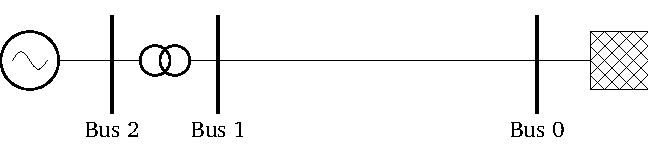
\includegraphics{tikz_graphics/images/smib_model.pdf}
    \vspace{12pt}
    \caption[]{\acf{SMIB} model for verification and validation of the Python framework; own figure after \autocite{machowski_2020,kundur_2022}}
    \label{fig:smib-model}
\end{figure}

\begin{table}[htb]
    \caption[Simulation Setup for validation of the $\Pi$-modeled transformer]{Simulation Setup for validation of the $\Pi$-modeled transformer; considering a transforming ratio $\underline{\vartheta} \neq 1$ and $\underline{\vartheta} \in \mathbb{C}$}
    \label{tab:smib-model}
    \vspace*{12pt}
    \centering
    \small
    \begin{tabularx}{\textwidth}{Xr}
        % \toprule
        \textbf{Parameter} & \textbf{Value} \\ \hline
        \toprule
        Generator inertia $H$ & 3.5 s \\
        Generator damping $D$ & 0.1 p.u. \\
        Generator resistance $R$ & 0.01 p.u. \\
        Generator reactance $X$ & 0.1 p.u. \\
        Transformer resistance $R$ & 0.01 p.u. \\
        Transformer reactance $X$ & 0.1 p.u. \\
        Transmission line resistance $R$ & 0.01 p.u. \\
        Transmission line reactance $X$ & 0.1 p.u. \\
        \bottomrule
    \end{tabularx}
\end{table}

Further, this model shall be slightly modified according to \autoref{fig:smib-model-mod}. 
A load is added at the secondary bus of the transformer, the rest of the system is kept. \autoref{tab:smib-model} already contains this modification.

\begin{figure}[htb!]
    \centering
    \vspace{12pt}
    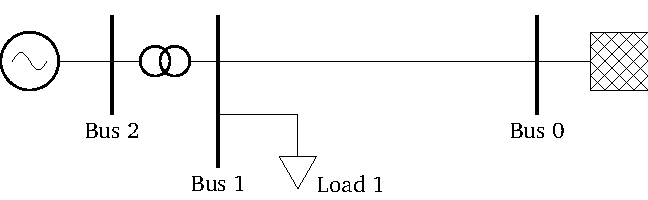
\includegraphics{tikz_graphics/images/smib_model_with_load.pdf}
    \vspace{12pt}
    \caption[]{Modified \acf{SMIB} model with additional load}
    \label{fig:smib-model-mod}
\end{figure}

\subsubsection{Simple Single Machine Load Model}

Following model is often recommended \quelle for easy voltage control studies, in explicit for \acsp{OLTC}. 
Similar to the \acs{SMIB} model, it consists from one synchronous generator, busses, and lines in a single branch. 
The \acs{IBB} is thus removed and changed to a load. 
This two element type o configuration allows for an easy analytical calculation of voltage stability and control. 
Although this thesis is focussing on \acs{OLTC} transformers, the model is extended with one in between. 
A single line representation is depicted in \autoref{fig:single-line-voltage-stability}.

\begin{figure}[htb!]
    \centering
    \vspace{12pt}
    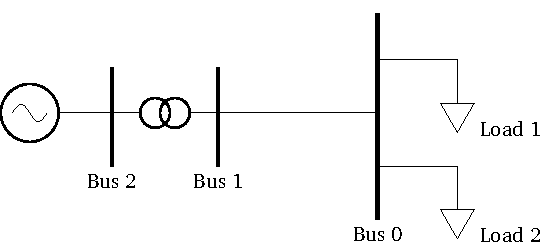
\includegraphics{tikz_graphics/images/sm_load_model.pdf}
    \vspace{12pt}
    \caption[Single line representation of a simple single machine load model]{Single line representation of a simple single machine load model; own illustration with characterstics from \quelle}
    \label{fig:single-line-voltage-stability}
\end{figure}

Further details about its configuration and simulation setup are included in \autoref{app:single-line-model}. 
It should be noted, that simple load models are not useful for simulation of this example network. 
Usually constant Z models are used as loads, therefore simulation results can be misleading and not showing desired effects or voltage instability mechanisms \quelle. 
% \commenting{The simulation framework is extended with XX types of load models, to satisfy the requirements of the single machine load model, and a connected stability assessment.}

% \subsubsection{IEEE Nine-Bus System}

% \subsubsection{Nordic Test System}

%%%%%%%%%%%%%%%%%%%%%%%%%%%%%%%
%%%%%%%%%%%%%%%%%%%%%%%%%%%%%%%
\section{Validation Steps}

Following section shall guide through the validation process.
Beginning with the new transformer $\Pi$-model, therefore lokking deeper into characteritic behavior dependent on the rated apparent power and the longitudinal ratio.
Proceeding with the three modeled control circuit and their behavior.
Lastly, some applied plausibilisations shall be done with the implemented voltage stability rating tools.

%%%%%%%%%%%%%%%%%%%%%%%%%%%%%%%
\subsection{Validation of the Modeled Transformer with Variable Tap Position}

As mentioned before, the base validation is concerning the basic transformer model.
For this, a parameter variation and comparison to the results from \textit{DIgSILENT PowerFactory} shall give a good representation of the accuracy.
The varied parameters are the apparent rated power $S_\mathrm{n}$ of the transformer, the longitudinal ratio $\vartheta$, the transformer reactance $X$, and the phase shifting angle $\phi$, resulting from the applied vector group.
The last two parameters are not included, because the transformer reactance is passively included in the ratio.
The reason for excluding the vector angle $\phi$ relies in the not congruent results.

\subsubsection{Variation of the Apparent Power}

\begin{figure}[htbp!]
    \centering
    \includegraphics[width=\linewidth]{development_files/validation/data/s_n_comp_errors.pdf}
    \caption[Model error comparison concerning the variation of the rated apparent power]{Absolute errors while comparing the tool \textit{diffpssi} with the software \textit{DIgSILENT PowerFactory}; One plot each for every parameter variation, concerning the errors for each bus}
    \label{fig:valid-s-errors}
\end{figure}

The rated apparent power $S_\mathrm{n}$ shall be varied in three steps acoording as described in \autoref{eq:variation-s-n}. 
The used grid model is the afore described \acs{SMIB} model. 
This is showing some predictable dynamics, but enabling a relative uncomplicated and easy to overview troubleshooting, if necessary.
The used grid parameters staying as described before, only the transformer apparent power is varied.
\begin{align}
    S_\mathrm{n} \in \{ 1100; 2200; 4400 \}~\mathrm{MVA} \label{eq:variation-s-n}
\end{align}
The used model for the comparative tool \textit{DIgSILENT PowerFactory} is as well included in the \textit{diffpssi} repository.
A plot of both results is depicted in \autoref{fig:valid-s-compl}
Looking deeper into one parameter, but plotting both tools in one diagram, \autoref{fig:valid-s-1100} in \autoref{app:add-validation-plots} is showing the results.
The three split diagrams account for each bus, where nearly no difference is obtainable.

Supporting this observation is the comparison of errors as illustrated in \autoref{fig:valid-s-errors}.
The error is not exceeding $0.005$ p.u. in any case.
One note to make here is, that due to the per unit nature of the calculation the initial values are often around $1$ p.u.
Therefore the seperate calculation of a relative error is neglected, as the absolute error is containing more information, and thus not surpassing the feel of relative nature.
Following this argumentation, the maximum relative error shall be around $0.05$ \% for this parameter variation.

\subsubsection{Variation of the Longitudinal Ratio}

\begin{figure}[htbp!]
    \centering
    \includegraphics[width=\linewidth]{development_files/validation/data/theta_comp_errors.pdf}
    \caption{Comparison of different varied parameters between \textit{diffpssi} and \textit{DIgSILENT PowerFactory}}
    \label{fig:valid-ratio-errors}
\end{figure}

In similar way as the validation approach for the rated apparent power, the longitudinal ratio shall be varied. 
Therefore the same network, with identical parameters is used, only that at this time the rated apparet power is fixed as well and the longitudinal ratio of the transformer is fixed during the simuatlion time according to following variation:
\begin{align}
    \vartheta \in \{ 0.9; 1.0; 1.1 \}~\mathrm{p.u} \label{eq:variation-ratio}
\end{align}
Looking into the results, in the same form as previously.
On the left side of \autoref{fig:valid-ratio-comp} is the result from the Python module \textit{diffpssi}, the right side is accounting for the validation tool \textit{DIgSILENT PowerFactory}.
The focussed comparison for the fixed ratio of $0.9$ p.u. is included in \autoref{app:add-validation-plots}.
As well \autoref{fig:valid-ratio-errors} is showing absoulte errors in the same manner.
The obtainable error for this case is comparably high, excluding for the reductive ratio of $0.9$ p.u.
This increasing with simulation time, to around a factor of 10 of the other errors. 
But still, this error is in a margin of lower than $1$ \%. 


%%%%%%%%%%%%%%%%%%%%%%%%%%%%%%%
\subsection{Parenthesis: Accountability of the Load Model}
\label{sec:validation-load-model}

\begin{figure}[htbp!]
    \centering
    \includegraphics[width=\linewidth]{development_files/validation/data/comparison_z_load.pdf}
    \caption[Comparison of the constant impedance model for each bus]{Comparison of the constant impedance model for each bus between the Python module \textit{diffpssi} and \textit{DIgSILENT PowerFactory}}
    \label{fig:z-comp}
\end{figure}

A static load model with quadratic dependency on the voltage had been implemented in the Python module before.
The load model can thus be classified as constant impedance model, or often referred as constant $\underline{Z}$ model \autocite{IEEELoadModeling_2022}. 
As this is playing a role in the chain of accumulating errors, following parenthesis shall give a feeling what contibution is generated through this load model.
For this evaluation the Single Line with Load model from \autoref{sec:networks} is used, with a load jump from $P=400\text{ MW}$ to $P=800\text{ MW}$ at the time stamp $1$ s.
The overall simulation time is set to $20$ s.
Other parameters are set as described in \autoref{sec:networks}.

\begin{figure}[htbp!]
    \centering
    \includegraphics[width=\linewidth]{development_files/validation/data/z_load_error.pdf}
    \caption[Absolute error comparison of the constant impedance model]{Absolute error of the already implemented constant impedance model over time; Accounted for both busses zero and one}
    \label{fig:z-load-error}
\end{figure}

\autoref{fig:z-comp} is showing the time series computation for each bus compared between both tools \textit{diffpssi} and \textit{DIgSILENT PowerFactory}.
Visible is the more extreme pronounciation of the overshoot and the convergence value over time of the Python package.
Looking at the absolute error comparison for each bus in \autoref{fig:z-load-error} showing a increase over time, and peak offsets of around $0.006$ p.u.
This accounts for an error lower than $1$ \% in this scenario.

%%%%%%%%%%%%%%%%%%%%%%%%%%%%%%%
\subsection{Validation of the OLTC Control Schemes}
\label{sec:validation-oltc-schemes}

To begin with this section of control scheme validation, the basic strategy accounted for all the considered models and verification setups.
The characterizations of the control loop feedbacks has already been carried out in the modeling chapter \autoref{sec:modeling-tap-changer-control}.
To validate the in-simulation behavior of the control loops, two different scenarios are accounted for the \acs{OLTC} and the \acs{FSM}.
First, the Simple Load against Machine grid is used with the declared parameters as in \autoref{sec:networks}.
To bring the system in a dynamic state, a load increase is added at the simulation time point $1$ s.
All differing values are pointed out in the validation result presentation later on.
Secondly, the more complex version of a \acs{SMIB} model with a connected load at the middle bus is used to account for a different scenario including a load flow direction change.
It would be expected, that neither \textit{DIgSILENT PowerFactory} or \textit{diffpssi} would be able to react on this supposed load flow direction change.

\subsubsection{Standard Discrete OLTC Control}

The first consideration for validation of the \acs{OLTC} control is the simple load model against a machine.
The applied load change is shifting the real power of the load from $P=400\text{ MW}$ to $P=800\text{ MW}$ at the simulation time $1$ s.

\begin{figure}[htbp!]
    \centering
    \includegraphics[width=\linewidth]{development_files/validation/data/comp_oltc_simple-load.pdf}
    \caption[Time Domain Result of the OLTC control scheme applied on the extended \acs{SMIB} network]{\acf{TDS} of the standard discrete \acs{OLTC} control scheme; Result of the extended or modified \acs{SMIB} model with additional load}
    \label{fig:comp-oltc-simple}
\end{figure}

When comparing the time series solution from \autoref{fig:comp-oltc-simple} for both bus voltages, one can obtain a similar course of the curves. 
Only a small deviation is visible, the tap changes of the \acs{OLTC} clearly visible and around the same times.
A similar picture is drawn, when loooking at the absolute error of this scenario in \autoref{fig:comp-oltc-error-simple}.
In the areas of time, where the switching occurs, peaks of errors are visible, showing just the less congruent development of bus voltages and switching.
After the half of the simulation time, a new (quasi-) stationary state is showign a static offset or error.
This error is around $0.005$ p.u., showing a slightly higher error than when looking at this scenario without the tap changing transformer in \autoref{sec:validation-load-model}.

\begin{figure}[htbp!]
    \centering
    \includegraphics[width=\linewidth]{development_files/validation/data/error_oltc_simple-load.pdf}
    \caption[Bus and Error Comparison for the standard discrete \acs{OLTC} scheme applied on the extended \acs{SMIB} model with load]{Comparison of the standard discrete \acs{OLTC} control scheme applied on the extended \acs{SMIB} model with additional load; One plot for each bus with data from \textit{diffpssi} and \textit{DIgSILENT PowerFactory}; Additional plot for showing the absolute error for each bus}
    \label{fig:comp-oltc-error-simple}
\end{figure}

Some blibla

\begin{figure}[htbp!]
    \centering
    \includegraphics[width=\linewidth]{development_files/validation/data/comp_oltc_ext-smib.pdf}
    \caption[Bus and Error Comparison for the standard discrete \acs{OLTC} scheme applied on the extended \acs{SMIB} model with load]{Comparison of the standard discrete \acs{OLTC} control scheme applied on the extended \acs{SMIB} model with additional load; One plot for each bus with data from \textit{diffpssi} and \textit{DIgSILENT PowerFactory}; Additional plot for showing the absolute error for each bus}
    \label{fig:comp-oltc-control-ex-smib}
\end{figure}

\begin{figure}[htbp!]
    \centering
    \includegraphics[width=\linewidth]{development_files/validation/data/oltc_ex-smib_signals.pdf}
    \caption[Internal signals of the \acs{OLTC} control in the extended \acs{SMIB} model]{Internal signals of the \acs{OLTC} control in the extended \acs{SMIB} model; a) the longitudinal transformer ratio $u_\mathrm{l}$ or mathematically referred as $\vartheta$, b) the deadband filtered voltage difference signal $v_\mathrm{dead}$}
    \label{fig:int-signals-ext-smib-oltc}
\end{figure}

\subsubsection{Fast Switching OLTC Control}

As described in the modeling chapter, specically \autoref{sec:modeling-tap-changer-control}, of the \acs{FSM} module control, two control methods are implemented.
First, as described in the paper of \textcite{burlakin_2024} with preferring the switching of the \acs{FSM}, and secondly the dependence on the function of tap skipping.
As only the last model is available in the comparative tool \textit{DIgSILENT PowerFactory}, only this can be compared and validated. 
The other control scheme is implemented similarly and used as well for futher studies.

\commenting{
    Due to some factors (which?), the control becomes more off the more states it has -> FSM seems not good, OLTC okay, Loads nearly identical.
    This means there must be differences within the static / dynamic time steps, the load model parameterization, The load model behavior, the model of the transformer itself, the discrecity of the transformer tap control etc.

    This means: Showing, that the control algorithmics is switching correctly, no matter what the result does look like at the bus voltages e.g.
}

%%%%%%%%%%%%%%%%%%%%%%%%%%%%%%%
\subsection{Voltage Stability Rating Plausibility}

\commenting{
    Place results here, looking at: off nominal tap ratio, and with off nominal phase shifting (e.g. $110^\circ$)

    Things to illustrate:
    \begin{enumerate}
        \item Validity of Top Branch Nose Curves: Analytical and PowerFactory; Simple Network and e.g. IEEE 9-bus 
        \item Analytical Validity OLTC ratio dependent Nose Curves
        \item Time Domain Projection: Dependence and Stability in transient scenarios vs. continous load increase; Dependence on Machine Controls; Dependence on Apparent Power Capacity of machine 
    \end{enumerate}
}

%%%%%%%%%%%%%%%%%%%%%%%%%%%%%%%
\section{Model Limitations and Improvements}

\section{Summary in Short and Simple Terms}